\section{Identification de la Dynamique}

Pour que ce qui va être présenté par la suite ait du sens, il est nécessaire de savoir dans quelles conditions nous travaillons.\\
Nos réponses sont basées sur un point de fonctionnement de $MV_0 = 50\%$, $DV_0 = 50\%$ et une sortie $PV_0 = 49.3^{\circ}$C. 
C'est à dire que la température obtenue sur $PV$ lorsqu'une puissance de chauffe de 50\% est appliquée sur les 2 chauffages est de 49.3°C en régime établi.

\subsection{Processus P(s)}

Appliquons un step $X(s) = \frac{1}{s}$ autour du point de fonctionnement (de 30\% à 70\%) lorsque le système se situe en régime établi pour analyser la "step response" $Y(s) = \frac{P(s)}{s}$.
\begin{figure}[h]
    \centering
    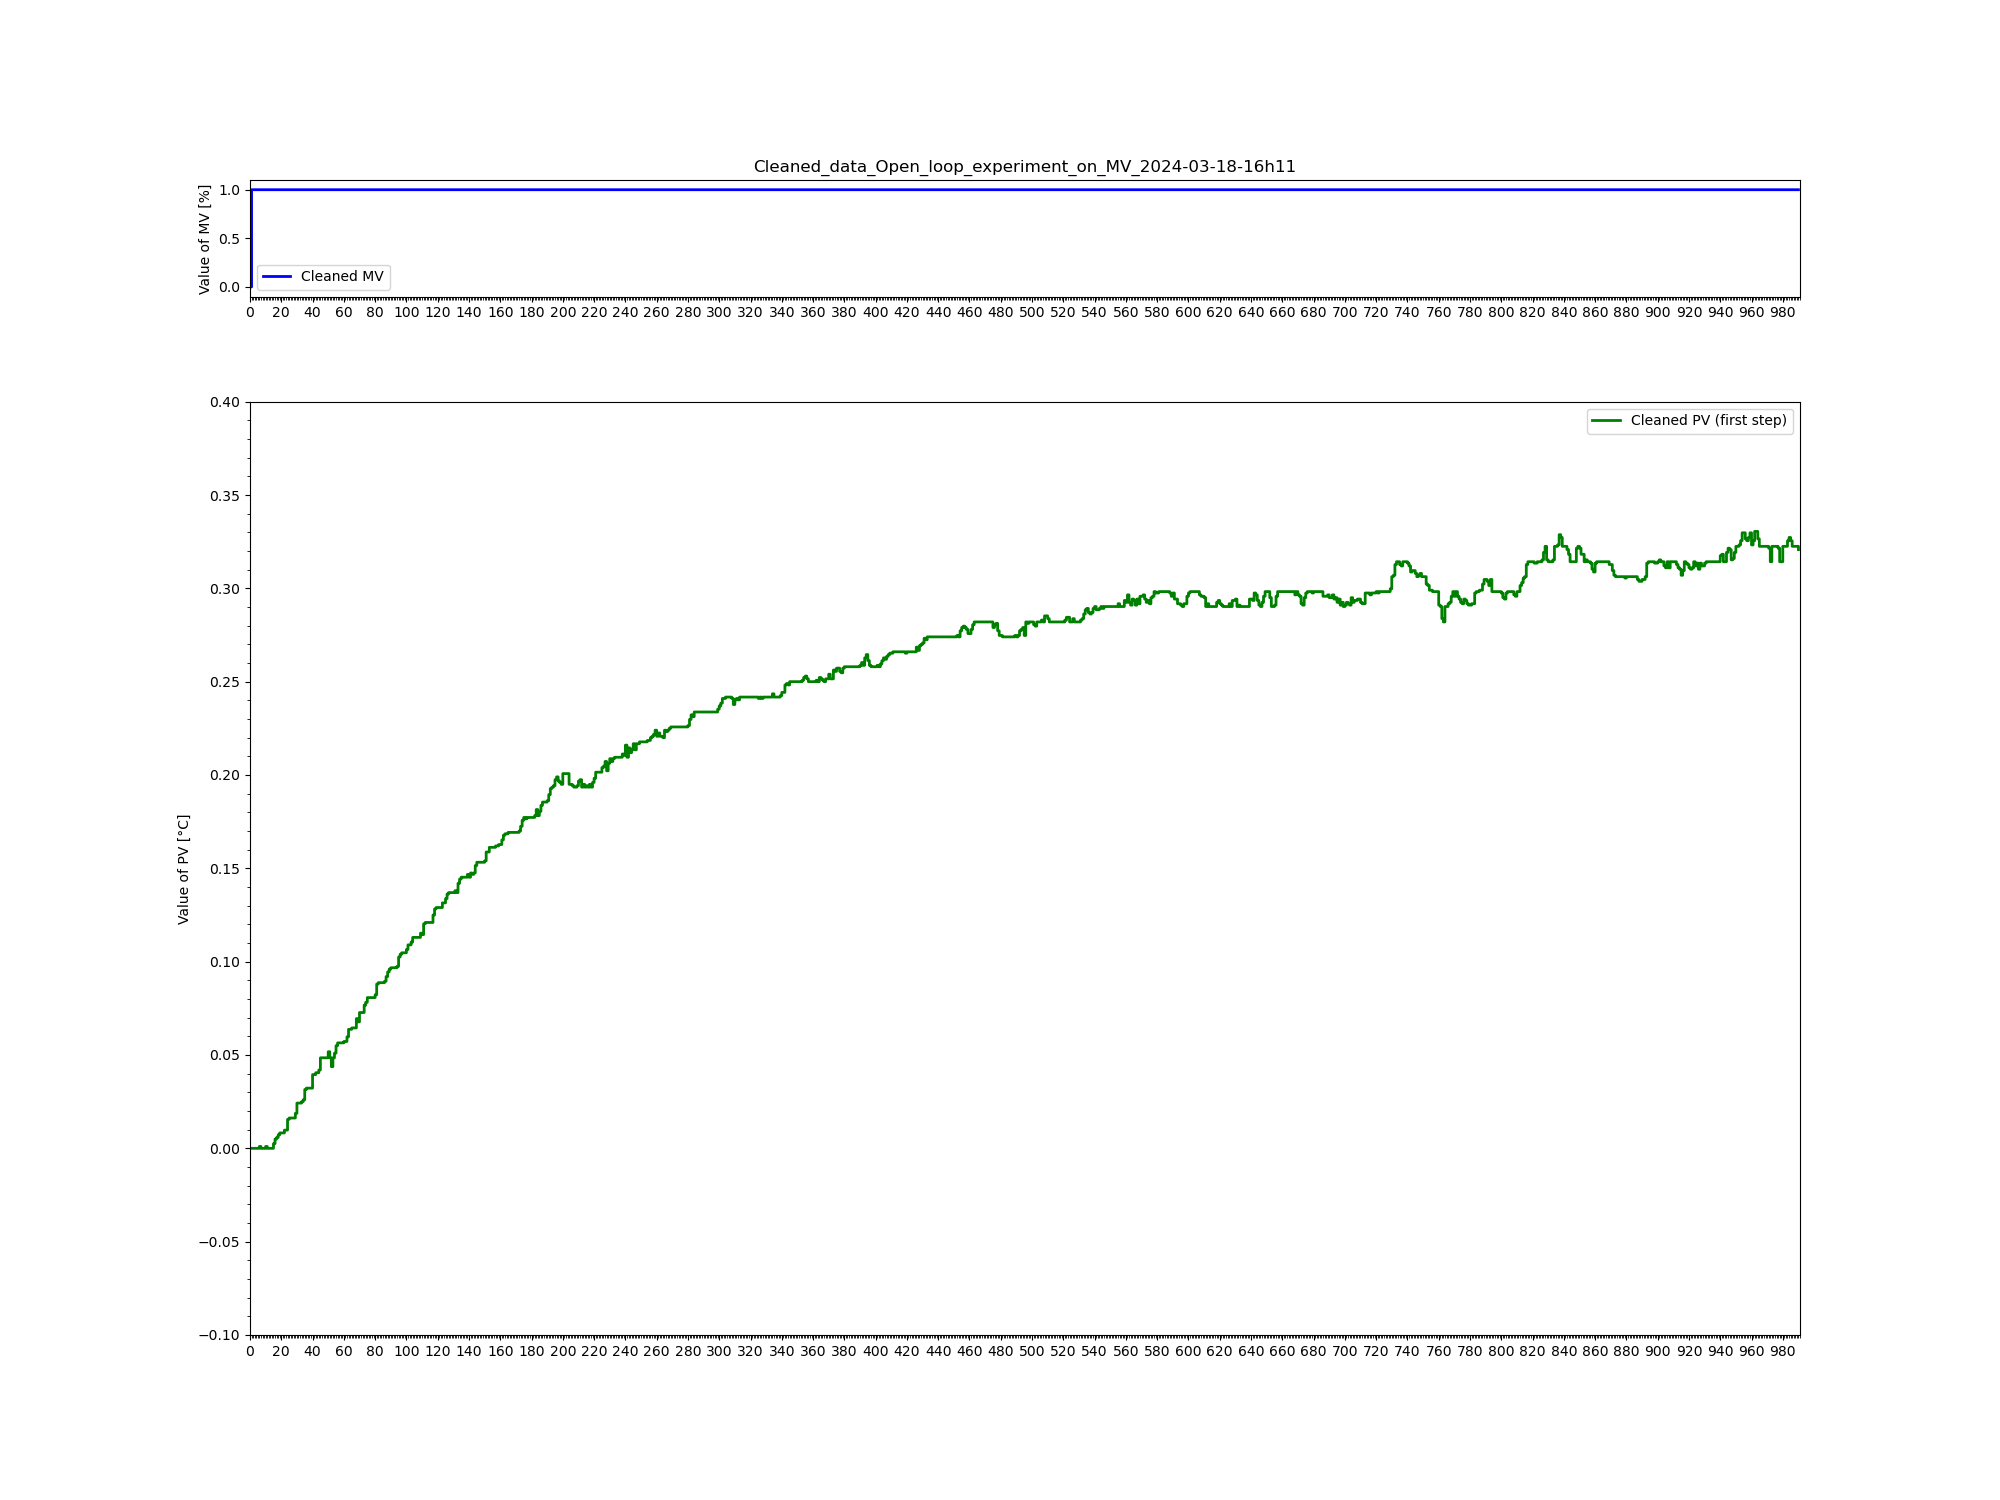
\includegraphics[width=0.9\textwidth]{../Plots/Graphical_methods_Cleaned_data_Open_loop_experiment_on_MV_2024-03-18-16h11.png}
    \caption{Réponse à un step sur MV}
    \label{fig:MV_step_response}
\end{figure}

Le graphique (Figure \ref{fig:MV_step_response}) obtenu permet (presque) d'affirmer que le processus est un système du $1^{e}$ ordre avec un délai. L'allure de la "step response" est donc $y(t) = K_p (1-e^{-t/T})u(t)$.

Le fichier \texttt{Identification.ipynb} permet de trouver les valeurs estimées de $K_P$, $T_1p$, $T_2p$ et $\theta_p$ qui vont par après nous servir à modéliser le Processus et la Perturbation de façon optimale, ainsi que les différentes méthodes d'approximations des modèles du $1^{e}$ et $2^{e}$ ordre.\\
Pour notre réponse du Processus, nous obtenons les valeurs suivantes pour un modèle du $2^{e}$ ordre :
\begin{align*}
    K_P &= 0.308 \\
    T_{1p} &= 183.819 \,s \\
    T_{2p} &= 3.292 \cdot 10^{-12} \,s \\
    \theta_p &= 20.015 \,s
\end{align*}
Et les valeurs suivantes pour un modèle du $1^{er}$ ordre :
\begin{align*}
    K_P &= 0.314 \\
    T_{p} &= 206.264 \,s \\
    \theta_p &= 12.999 \,s
\end{align*}
On remarque directement que $T_{2p}$ est négligeable par rapport à $T_{1p}$, et permet donc de confirmer que le processus agit comme un système du $1^{er}$ ordre avec délai :
\begin{equation}
    \hat{P}(s) = \frac{K_P\,e^{-\theta_p s}}{(T_{1p}s + 1)(T_{2p}s + 1)} \approx \frac{K_P\,e^{-\theta_p s}}{T_{1p}s + 1}
\end{equation}

\subsubsection{Approximation graphique du modèle pour MV}

Il est également possible de déterminer la dynamique du Processus graphiquement sur base de la Figure \ref{fig:MV_step_response}.
Nous obtenons les paramètres $K_P$, $T_u$, $T_g$, $t_1$, $t_2$ et $a$ dont la détermination est expliquée en Annexe \ref{appendix:MV_graphical_method} :
\begin{align*}
    K_P &= 0.305 \\
    T_u &= 17 \,s \\
    T_g &= 211 \,s \\
    t_1 &= 95 \,s \\
    t_2 &= 133 \,s \\
    a &= 0.1
\end{align*}
Ces paramètres servirons à utiliser les méthodes classiques d'approximation du modèle, à savoir le modèle de \textbf{Broida}, \textbf{Van Der Grinten} et \textbf{Strejc}.

\subsubsection{Modèle de Broida (FOPDT)}
Ce modèle consiste à approximer le Processus par un système du $1^{er}$ ordre avec délai de la forme :
\begin{equation*}
    P_B(s) = \frac{K_P\,e^{-\theta s}}{T s + 1}
\end{equation*}
Le \underline{$1^{er}$ modèle} de Broida est obtenu en définissant la constante de temps $T$ et le délai $\theta$ comme suit :
\begin{center}
    $T = T_g = 211\,s$ \, et \, $\theta = T_u = 17\,s$
\end{center}
Le \underline{$2^{e}$ modèle} de Broida est obtenu en définissant la constante de temps $T$ et le délai $\theta$ comme suit :
\begin{center}
    $T = 5.5\,(t_2 - t_1) = 209\,s$ \, et \, $\theta = 2.8\,t_1 - 1.8\,t_2 = 26.60\,s$
\end{center}

\subsubsection{Modèle de van der Grinten (SOPDT)}
Ce modèle consiste à approximer le Processus par un système du $2^{e}$ ordre avec délai de la forme :
\begin{equation*}
    P_{vdG}(s) = \frac{K_P\,e^{-\theta s}}{(T_1 s + 1)(T_2 s + 1)}
\end{equation*}
$T_1$, $T_2$ et $\theta$ sont obtenus comme suit :
\begin{align*}
        T_1 &= T_g\,\frac{3ae - 1}{1 + ae} = -30.61\,s\\[4pt]
        T_2 &= T_g\,\frac{1 - ae}{1 + ae} = 120.81\,s\\[4pt]
        \theta &= T_u - \frac{T_1T_2}{T_1 + 3T_2} = 28.15\,s
\end{align*}
Nous constatons que la $1^{e}$ constante de temps $T_1$ est négative, ce qui est physiquement impossible! 
Il n'est cependant pas étonnant d'obtenir ce résultat étant donné que le Processus est un système du $1^{er}$ ordre avec délai.
Un modèle du $2^{e}$ ordre tel que van der Grinten n'est donc pas adapté pour approximer notre Processus et ne sera donc pas représenté par après.

\subsubsection{Modèle de Strejc}
Ce modèle consiste à approximer le Processus par un système du $n^{e}$ ordre avec des pôles et constantes de temps identiques de la forme :
\begin{equation*}
    P_S(s) = \frac{K_P\,e^{-\theta s}}{(T s + 1)^n}
\end{equation*}
L'ordre $n$ est obtenu avec la Table \ref{tab:Strejc_order} :
\begin{table}[H]
    \centering
    \begin{tabular}{|c|c|c|} 
        \hline
        Order $n$ & $T_{u_{th}}/T_g$ & $T_g/T$ \\
        \hline
         & $a_n$ & $b_n$ \\
        \hline
        1 & 0.00 & 1.00 \\
        \hline
        2 & 0.10 & 2.72 \\
        \hline
        3 & 0.22 & 3.69 \\
        \hline
        4 & 0.32 & 4.46 \\
        \hline
        5 & 0.41 & 5.12 \\
        \hline
        6 & 0.49 & 5.70 \\
        \hline
        7 & 0.57 & 6.23 \\
        \hline
    \end{tabular}
    \caption{Ordre $n$ du modèle de Strejc en fonction de $a_n$ et $b_n$}
    \label{tab:Strejc_order}
\end{table}
Nous avons que $T_u/T_g = 0.08$ et donc ce situe à $a_1 \leq 0.08 < a_2$, ce qui nous donne un ordre $n = 1$. $a_n$ vaut alors 0.00 et $b_n$ vaut 1.00.
La constante de temps $T$ et le délai $\theta$ vont être au final trouvés directement avec les valeurs de $T_g$ et $T_u$ comme le modèle de Broida :
\begin{align*}
    T = \frac{T_g}{b_n} = T_g = 211\,s\\
    \theta = T_u - a_n T_g = T_u = 17\,s
\end{align*}

\subsubsection{Comparaison des modèles d'approximation}

\begin{figure}[H]
    \centering
    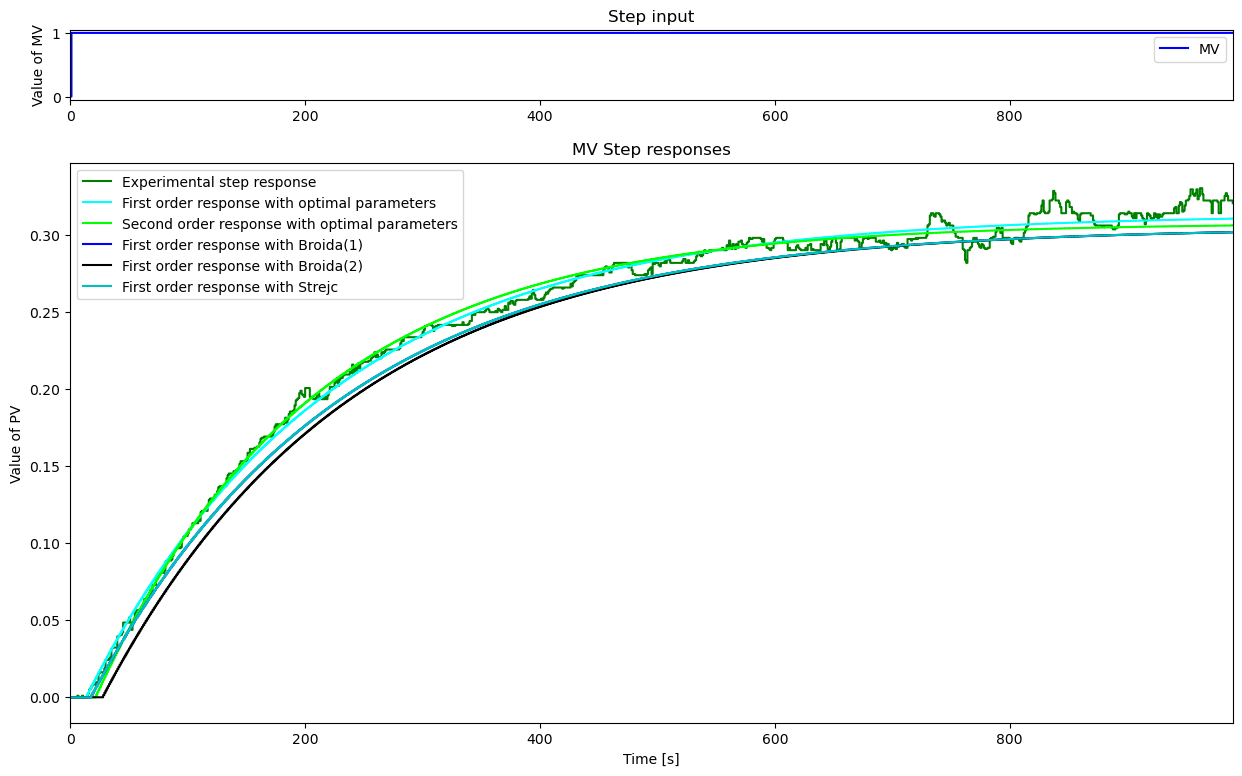
\includegraphics[width=0.9\textwidth]{../Plots/MV_Approximations_comparison_time.png}
    \caption{Approximations de la réponse temporelle d'un step sur MV}
    \label{fig:MV_approximation_comparison_time}
\end{figure}
\begin{figure}[H]
    \centering
    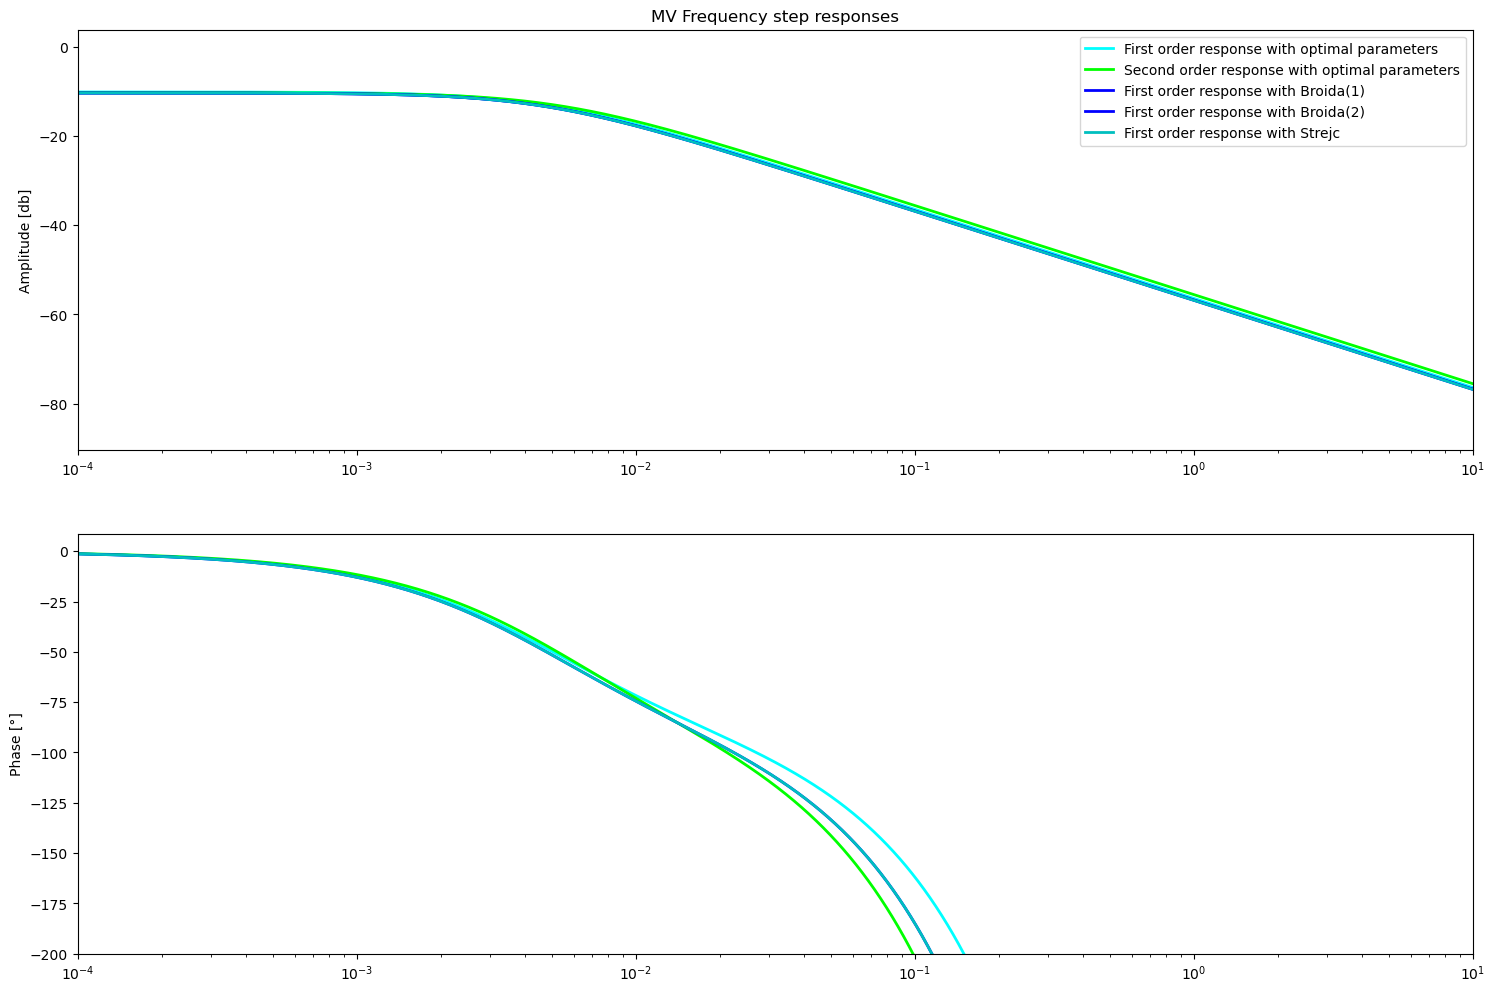
\includegraphics[width=0.9\textwidth]{../Plots/MV_Approximations_comparison_frequency.png}
    \caption{Approximations de la réponse fréquentielle d'un step sur MV}
    \label{fig:MV_approximation_comparison_frequency}
\end{figure}

La Figure \ref{fig:MV_approximation_comparison_time} montre les différentes réponses d'un step sur MV pour chacun des modèles décrits au-dessus (à l'exeption du modèle de van der Grinten).
Elles représentent toutes bien une réponse du $1^{e}$ ordre avec délai, et restent assez proches les unes des autres.
Les modèles commencent tous avec un délai similaire et terminent en régime établi à environ le même gain statique $K_P$.\\
Cependant, on distingue tout de même les modèles avec paramètres optimaux des modèles graphiques.
Les paramètres optimaux ont été trouvés par un algorithme de minimisation de l'erreur, tandis que les paramètres graphiques ont étés trouvés par une méthode graphique dont la précision est à prendre avec recul.
\par
La Figure \ref{fig:MV_approximation_comparison_frequency} nous permet ensuite de comparer les réponses fréquentielles des différents modèles.
La première observation est que tous les modèles sont pratiquement supperposés en terme de gain.
En basses fréquences, ils atteignent bien un gain de $K_P = -10\,dB = 0.3$ et en hautes fréquences, ils subissent tous une pente de $-20\,dB$/décade.
On peut également confirmer que la réponse du $2^{e}$ ordre avec paramètres optimaux est bien en fait un $1^{er}$ ordre en raison d'une constante de temps négligeable.\\
En ce qui concerne la phase, on obtient bien une allure à la quelle on s'attendait pour un système du $1^{er}$ ordre avec délai, à savoir une phase qui tends vers l'infini (en négatif) lorsque la fréquence tends vers l'infini.
Nous constatons que la courbe bleue (premier ordre optimal) et la courbe verte (second ordre optimal) dévient plus la fréquence augmente. Cela peut être expliqué par la différence entre les deux délais $\theta_p$ qui sont de 13 et 20 secondes respectivement.
En effet, pour atteindre une même phase représenté par $\theta s = j\theta\omega$, il faudra une fréquence plus élevée pour le modèle du $1^{er}$ ordre que pour le modèle du $2^{e}$ ordre. 

%---------- Identification de la Dynamique de la Perturbation ----------%
\subsection{Perturbation D(s)}

Nous appliquons maintenant un step sur DV pour observer la réponse du système à une perturbation.
\begin{figure}[H]
    \centering
    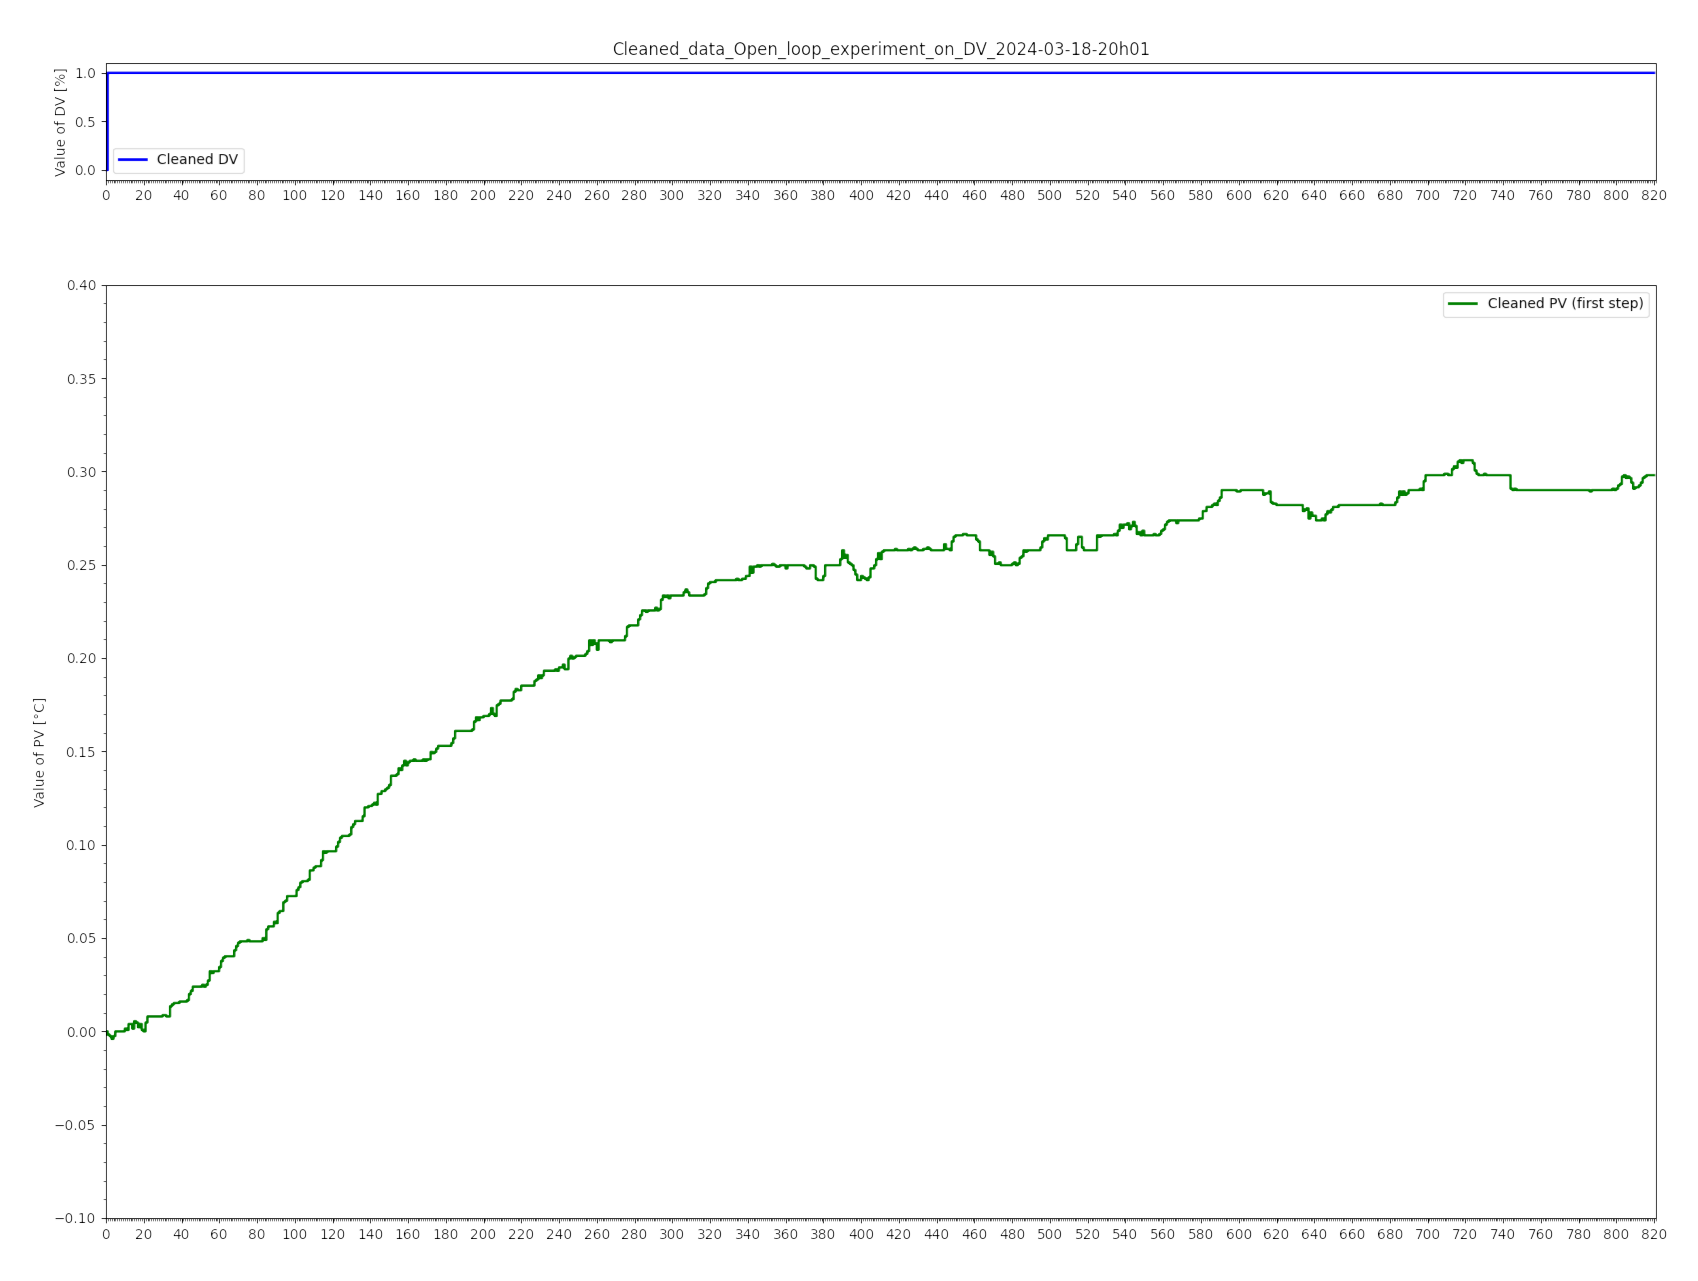
\includegraphics[width=0.9\textwidth]{../Plots/Graphical_methods_Cleaned_data_Open_loop_experiment_on_DV_2024-03-18-20h01.png}
    \caption{Réponse à un step sur DV}
    \label{fig:DV_step_response}
\end{figure}

Étant donné l'allure du graphe (Figure \ref{fig:DV_step_response}), et en particulier le point d'inflexion aux alentours de 80 secondes, nous pouvons estimer que la perturbation se comporte comme un système du $2^{e}$ ordre avec délai de la forme :
\begin{equation}
    \hat{D}(s) = \frac{K_D\,e^{-\theta_d s}}{(T_{1d}s + 1)(T_{2d}s + 1)}
\end{equation}
En effet, nous obtenons grâce au fichier \texttt{Identification.ipynb}, les valeurs optimales suivantes pour un modèle du $2^{e}$ ordre :
\begin{align*}
    K_D &= 0.295 \\
    T_{1d} &= 182.255 \,s \\
    T_{2d} &= 13.184 \,s \\
    \theta_d &= 28.999 \,s
\end{align*}
Et les valeurs suivantes pour un modèle du $1^{er}$ ordre :
\begin{align*}
    K_D &= 0.296 \\
    T_{d} &= 184.880 \,s \\
    \theta_d &= 40.136 \,s
\end{align*}
Les valeurs obtenues pour $T_{1d}$ et $T_{2d}$ nous permettent de confirmer que la perturbation peut se comporter comme un système du $2^{e}$ ordre.

\subsubsection{Comparaison des modèles avec paramètres optimaux}

\begin{figure}[H]
    \centering
    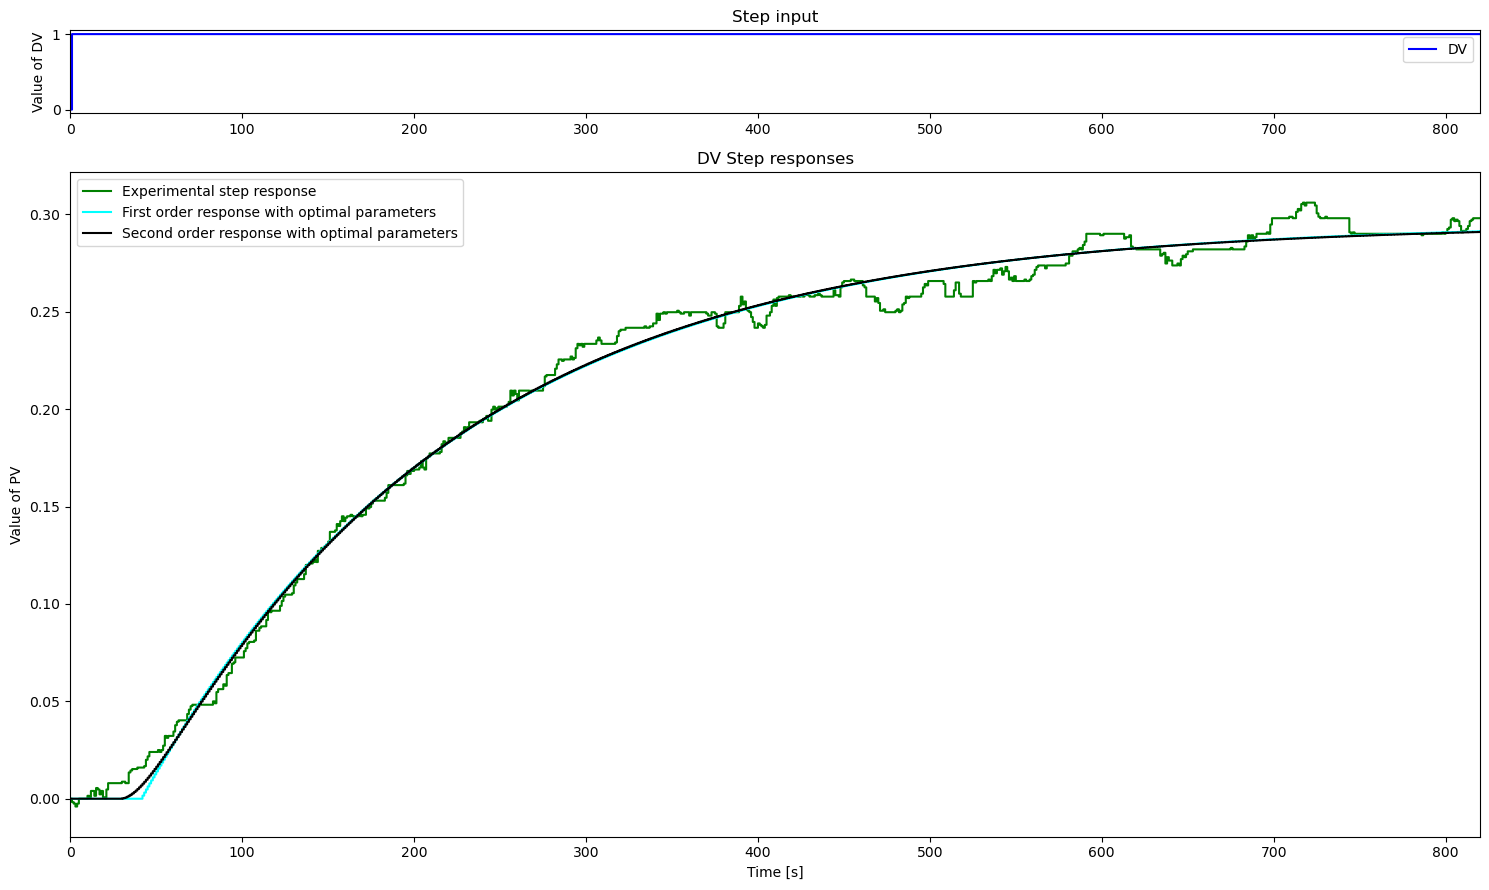
\includegraphics[width=0.9\textwidth]{../Plots/DV_Approximations_comparison_time.png}
    \caption{Approximations de la réponse temporelle d'un step sur DV}
    \label{fig:DV_approximation_comparison_time}
\end{figure}
Il est clair que la Figure \ref{fig:DV_approximation_comparison_time} montre que les modèles du $1^{er}$ et $2^{e}$ ordre avec paramètres optimaux sont très proches l'un de l'autre.
La seule différence réside en la décomposition du délai du $1^{er}$ ordre en un délai et une constante de temps $T_{2d}$ pour le $2^{e}$ ordre.
L'ajout de cette constante de temps permet de mieux modéliser la réponse expérimentale du système à une perturbation.
\begin{figure}[H]
    \centering
    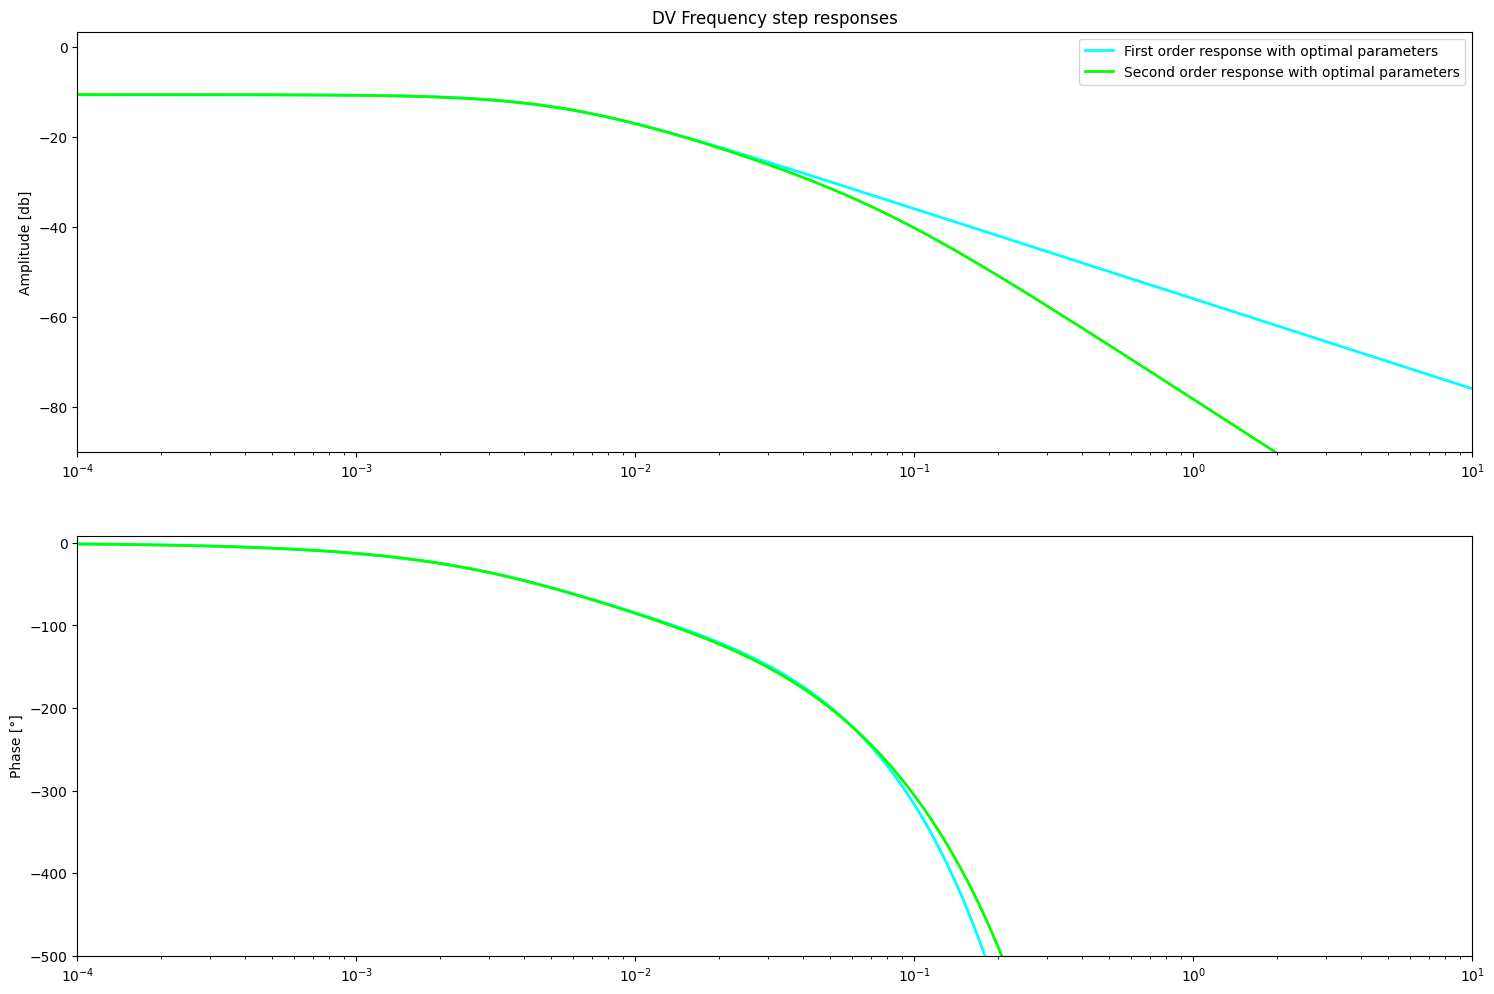
\includegraphics[width=0.9\textwidth]{../Plots/DV_Approximations_comparison_frequency.png}
    \caption{Approximations de la réponse fréquentielle d'un step sur DV}
    \label{fig:DV_approximation_comparison_frequency}
\end{figure}
Pouvant modéliser la perturbation comme un système du $1^{er}$ ou $2^{e}$ ordre avec délai, la réponse fréquentielle (Figure \ref{fig:DV_approximation_comparison_frequency}) est différente pour les deux modèles.
À hautes fréquences, le modèle du premier ordre possède une pente de $-20\,dB$/décade tandis que le modèle du second ordre possède une pente de $-40\,dB$/décade.
Le gain à basses fréquences vaut bien également $K_P = -10\,dB = 0.3$.\\
La phase, comme pour la partie Processus, tends vers l'infini (en négatif) lorsque la fréquence tends vers l'infini et dévie entre les deux modèles à hautes fréquences.
Cela peut être expliqué par la différence entre les deux délais $\theta_p$ qui sont cette fois de 40 secondes pour le premier ordre et 29 secondes pour le second ordre.
Le délai du sencond ordre étant cette fois plus petit, nous avons le comportement opposé : pour atteindre une même phase représenté par $\theta s = j\theta\omega$, il faudra une fréquence plus élevée pour le modèle du $2^{e}$ ordre que pour le modèle du $1^{er}$ ordre. 